\documentclass[UTF8]{book}

\usepackage[T1]{fontenc}
\usepackage{bookmark}
\usepackage{ctex} %这是中文latex必需品
\usepackage{lipsum}
\usepackage{amsmath, amsthm, amssymb, amsfonts,mathrsfs} %latex写数学的必需品
\usepackage{thmtools} %定理环境的工具
\usepackage{graphicx} %图片设置的工具
\usepackage{setspace}
\usepackage{geometry}
\usepackage{float} %设置图片位置
\usepackage{hyperref}
\usepackage[utf8]{inputenc}
\usepackage[english]{babel}
\usepackage{framed}
\usepackage[dvipsnames]{xcolor}
\usepackage{tikz-cd} %用tikz画图的工具
\usepackage[most]{tcolorbox}
\usepackage{enumerate} %序号
\usepackage[center]{titlesec}

\usetikzlibrary{positioning}

\usepackage{pgfplots}
\pgfplotsset{compat=newest}

\tcbuselibrary{theorems}
\tcbuselibrary{breakable}


%定义颜色,可以根据需求自己修改
\colorlet{LightGray}{White!90!Periwinkle}
\colorlet{LightOrange}{Orange!15}
\colorlet{LightGreen}{Green!15}
\colorlet{Lightblue}{Blue!15}
\colorlet{Lightpurple}{Purple!15}
\colorlet{LightRed}{Red!15}
\colorlet{LightYellow}{Yellow!15}
\colorlet{LightCyan}{Cyan!15}
\colorlet{LightAquamarine}{Aquamarine!15}
\colorlet{LightCadetBlue}{CadetBlue!15}

\newcommand{\HRule}[1]{\rule{\linewidth}{#1}}

\newtheorem{corollary}{Corollary}[section]
\newenvironment{solution}{{\noindent\it Solution.} }{\hfill $\square$\par}

\declaretheoremstyle[name=Theorem,]{thmsty}
\declaretheorem[style=thmsty,numberwithin=section,refname={定理}]{theorem}
\tcolorboxenvironment{theorem}{colback=LightGray,breakable,before upper app={\setlength{\parindent}{2em}}}

\declaretheoremstyle[name=Definition,]{thmsty}
\declaretheorem[style=thmsty,numberwithin=section,refname={定义}]{definition}
\tcolorboxenvironment{definition}{colback=LightCyan,breakable,before upper app={\setlength{\parindent}{2em}}}

\declaretheoremstyle[name=Remark,]{thmsty}
\declaretheorem[style=thmsty,numberwithin=section,refname={注记}]{remark}
\tcolorboxenvironment{remark}{colback=LightRed,breakable,before upper app={\setlength{\parindent}{2em}}}

\declaretheoremstyle[name=Lemma,]{thmsty}
\declaretheorem[style=thmsty,numberwithin=section,refname={引理}]{lemma}
\tcolorboxenvironment{lemma}{colback=Lightblue,breakable,before upper app={\setlength{\parindent}{2em}}}

\declaretheoremstyle[name=Corollary,]{thmsty}
\declaretheorem[style=thmsty,numberwithin=section,refname={推论}]{Corollary}
\tcolorboxenvironment{corollary}{colback=Lightpurple,breakable,before upper app={\setlength{\parindent}{2em}}}

\declaretheoremstyle[name=Proposition,]{prosty}
\declaretheorem[style=prosty,numberwithin=section,refname={命题}]{proposition}
\tcolorboxenvironment{proposition}{colback=LightOrange,breakable,before upper app={\setlength{\parindent}{2em}}}

\declaretheoremstyle[name=Example,]{prosty}
\declaretheorem[style=prosty,numberwithin=section,refname={例}]{example}
\tcolorboxenvironment{example}{colback=LightGreen,breakable,before upper app={\setlength{\parindent}{2em}}}

\declaretheoremstyle[name=Exercise,]{prosty}
\declaretheorem[style=prosty,numberwithin=chapter]{exercise}
\tcolorboxenvironment{exercise}{colback=LightAquamarine,breakable,before upper app={\setlength{\parindent}{2em}}}

\declaretheoremstyle[name=Hint \& Answer,]{prosty}
\declaretheorem[style=prosty,numberwithin=chapter]{answer}
\tcolorboxenvironment{answer}{colback=LightCadetBlue,breakable,before upper app={\setlength{\parindent}{2em}}}

\makeatletter
\newcommand{\rmnum}[1]{\romannumeral #1}
\newcommand{\Rmnum}[1]{\expandafter\@slowromancap\romannumeral #1@}
\makeatother %罗马数字的简洁打法

% 修改 Chapter 为 Lecture

\titleformat{\chapter}{\raggedright\Huge\bfseries}{Lecture \thechapter}{1em}{}
\titleformat{\section}{\raggedright\Large\bfseries}{\,\thesection\,}{1em}{}
\titleformat{\subsection}{\raggedright\large\bfseries}{\,\thesubsection\,}{1em}{}



\setstretch{1.2}
\geometry{
    textheight=9in,
    textwidth=5.5in,
    top=1in,
    headheight=12pt,
    headsep=25pt,
    footskip=30pt
}

% 设置 PDF 文件信息
%\hypersetup{
%	pdfauthor = {章梓杭},
%	pdftitle = {巴猪数学讲义 第一卷:数学分析},
%	pdfkeywords = {Analysis},
%	CJKbookmarks = true}

% ------------------------------------------------------------------------------

\begin{document}

% ------------------------------------------------------------------------------
% 封面设计如下:
% ------------------------------------------------------------------------------

%\setCJKfamilyfont{coverfont}{SIMKAI.TTF}	% 设置书名字体
%\setCJKfamilyfont{cover-author-font}{SIMSUN.TTF}	% 设置作者字体

% 设置标题样式

\begin{titlepage}
    \vspace*{10em}
\begin{center}
    \zihao{0} % 一号字大小,可根据需要调整
    \textbf{\songti 高等代数选讲} \\ % 加粗宋体显示“高等代数”
    \vspace{4em} % 增加一些垂直间距
    \zihao{4} % 四号字大小,可根据需要调整
    作者: ZZH \\ % 第二行写作者
    \vspace{10em} % 增加垂直间距

    % 页面下方写免责声明
    \zihao{5} % 五号字大小,可根据需要调整
    本讲义使用于 HEO 高等代数\Rmnum{2} 课程中, \\
    内容由 \LaTeX 编译, 图片使用 GeoGebra 绘制. \\
    参考多部书目, 仅用作学习讨论和笔记需求. 如有错误, 欢迎指正. \\
    使用时间 2025/3/3\\

    最后编译时间 \today\\
\end{center}

\end{titlepage} 

\newpage

\vspace*{5em}

每逢拾笔, 愿母亲安康. 

本笔记摘选自 巴猪数学讲义: 第二卷 高等代数. 

谨以彼书赠与女友与巴猪的陪伴. 

祝诸位在数学上逢见挚爱. 

\vspace*{5em}

摘自 Grassmann 扩张论. 您的理论如今已是大学入学必学的课程. 

\begin{quotation}
    \kaishu
    我始终坚信我在此科学上所付出的劳动不会白费, 它耗尽了我生命中最重要的阶段, 
    让我付出了超常的努力. 我当然知道我给出的这门科学的形式还不完善, 
    它一定是不完善的. 但是, 我知道而且有义务在此声明 (可能有人会认为我很狂妄), 
    即使这一成果再过十七年或更长时间还不被使用, 也没有真正融入到科学的发展之中, 
    它冲出遗忘的尘埃现身的时候也一定会到来, 现在沉睡着的思想结出硕果的那一天一定会到来. 
    我知道, 如果我今天还不能 (如我至今徒劳地期望那样) 把学者们吸引到我的周围, 
    用这些思想帮助他们成果累累, 促使其进步, 丰富其学识, 
    那么这种思想在将来一定会重生, 或许以另一种新形式, 与时代发展水乳交融. 
    因为真理是永恒不灭的. 
    \songti
\end{quotation}

\vspace*{5em}

摘自 Grothendieck 丰收与播种. 愿数学的远端没有硝烟. 

\begin{quotation}
    
    \kaishu   
    我可以用同样的坚果意象来说明第二种方法: 
    
    第一种类比: 
    我首先想到的是将坚果浸泡在某种软化液体中——为何不直接用水呢? 
    你偶尔摩擦坚果以促进液体渗透,其余时间则静待其变. 
    经过数周甚至数月, 外壳逐渐变得柔软——当时机成熟, 仅需用手轻轻一压, 
    它便会如完美成熟的牛油果般自然裂开! 

    几周前, 我的脑海中闪现了另一幅图像. 
      
    那片等待被理解的未知, 仿佛一片坚硬的土地或泥灰岩, 抗拒着侵入\dots
    而海水无声无息地悄然上涨, 看似毫无动静, 潮水遥远得几乎听不见声响\dots 
    但它终将温柔包裹住那顽固的物体. 
    
\end{quotation}

代数就是这片 Rising Sea. 

\chapter{绪论: 代数学引论}


在小学时, 当加减乘除简单的算术已经炉火纯青之时, 无数孩童都会遭到一记重拳, 
以抽象的动机和几乎穷举的标准解法让人瞠目结舌的, \textbf{鸡兔同笼问题}. 
迄今为止,在社交媒体上也经常能够看到很多家长在辅导孩童作业的时候, 被鸡兔同笼
问题难倒, 笔者本人也有小学初中问题不会转而去询问父母的经验, 只见家长
看了看, 列了个方程, 几下就出来了, 随即就是一整晚都想不到这些题目究竟如何
用小学初中的方法解决. 

小学奥数自是有趣的, 笔者于小学时期经常喜欢借阅图书馆中的数学游戏一类的书目, 
可惜的是, 笔者阅读的时候就和读推理小说一样, 想都不想地直接过去了. 
但是现在想来, NP 完全的\textbf{邮差问题}与
图论诞生的\textbf{戈尼斯堡七桥问题}, 竟然早早地就在
十岁的脑海里留下了印象. 
这就是启蒙教育的魅力, 有些非常开放式的内容, 有些底层原理或许非常复杂的问题, 
有些不是照着既定算式固定模式的套路计算就能得到解答的问题, 却能够
让还没有多少算力的大脑去觉醒出 "数学的直觉". 

是的, 就好像在尝试做了几个数独之后就能够反应过来怎样的检索方式会让问题变得
明了; 玩了几次扫雷之后隐隐地发掘着背后是否有通解的固定算法; 
背多了平方表之后发现平凡差是一个奇数列. 
这并非是为了高中能把函数题解下去生硬地套着 L'Hopital 法则, 
结果上了大学接触了高等数学又全然不顾着微分中值定理以及 Taylor 公式的闪耀. 
所谓的数学启蒙, 或许就是被指引走到那扇虚掩着的门前方, 
不知道推开门是多少年后的事, 但是推开门的那一刹那, 却发现自己根本不需要
发动任何力量: 前面走过的那些路已足够让你流入那广袤的新海洋. 

我们理应是这样地迎接来了代数. 初中的方程, 高中的函数, 让呼之欲出的一切
清晰明了.

我们也将一直这样去走向那些虚掩的门, 等待一个时日, 推开它们. 

\section{早期代数: 于方程原野上对未知量的追逐}
%这里介绍一些代数的简要历史发展
现实应用对方程求解的需求源源不断, 因此, 早期的数学往往是在追求对那些
各式各样的方程的求解方法. 先追求能不能算出正确的答案来, 再追求有没有更快的
算法, 进而由这样的过程认识到数学的本质. 

\subsection{线性方程组: Gauss-Jordan 消元法}
%简单地叙述以下 Gauss 消元法的思想即可
Gauss-Jordan 消元法往往是作为高等代数的导入放在入口处的. 
一来它看似简单甚至有点显然的过程解决了一个非常大的问题, 
二来它直接将我们引向了矩阵. 

% 顺便,我们在此发现矩阵很适用
没错, 最早的矩阵仅仅是为了方便记录线性方程组而存在的, 甚至行列式的出现都比
矩阵要早得多. 

\subsection{多项式方程: 对求根公式的追求}
%这里推导出 三次方程和四次方程的求根公式
除了普通的线性方程和线性方程组, 多次方程也就是所谓的多项式方程也占据着很重要
的部分. 

我们初中就学习过二次方程 $ a x^2 + b x + c = 0 $ 的求根公式
\begin{equation}
    x = \frac{-b \pm \sqrt{b^2 - 4ac}}{2a},
\end{equation}, 
通过 Vieta 定理或是对二次函数的观察都很容易得到这个结果, 
并且通过对这个公式中的判别式 $\Delta =  \sqrt{b^2 - 4ac}$ 的思考
也引导我们去发现复数的存在. 

那么一个很朴素的问题就来了, 三次, 四次, 甚至更高次方程的求根公式是什么? 

首先, 观察我们的二次方程求根公式, 那里是有冗余的, 即我们没有必要去保留
二次项前面的系数, 我们可以通过等号两边同时除以 $a$ 将系数减少一个, 这样
也会让我们的求根公式更加简单, 并且结果也是不变的.

即, 对于首 1 (monic) 的二次方程 $ x^2 + px + q = 0 $, 我们有求根公式
\begin{equation}
    x = \frac{-p \pm \sqrt{p^2 - 4q}}{2}.
\end{equation}

同样的事情我们可以做到三次方程和四次方程中, 在本文中我们假设它们都是首 1 的. 

我们先设三次方程为 $F(X) = X^3+aX^2+bX+C=0$. 
如果我们采用一个线性变换 $ X = x-b/3 $, 
则可以发现方程的次高项被消去了, 方程变为了 $f(x) = x^3 + qx + r$. 
假如我们解出了 $x$, 则 $x-b/3$ 自然会成为原方程 $F(X)$ 的一个根. 
这样, 我们又进一步将三次方程的系数压缩至两个了. 

\begin{exercise}
    对于一般的首 1 多项式方程 $f(x) = x^n + a_1x^{n-1} + 
    \cdots + a_{n-1}x + a_n$ 是否可以通过线性变换消去次高项系数?
\end{exercise}

\begin{theorem}
    \textbf{三次方程求根公式} 三次方程 $f(x) = x^3 + qx + r$ 的三个根
    分别为 $$ g + h , \omega g + \omega ^2 h , \omega^2 g + \omega h, $$
    其中, $ g^3 = (-r + \sqrt{R})/2, h = -q/3g, R = r^2 + 4q^3/27, $
    并且
    $\omega = (-1+i\sqrt{3})/2 $ 是三次单位根. 
    ($\omega^3=1 , (\omega^2)^3 =1$) 
\end{theorem}

乍看之下这个求根公式乱糟糟的, 但只要知道这个证明过程就完全对这些字母是从哪来的
一清二楚了. 

下面是这个公式的展开式
$$ x_{1}=\sqrt[3]{-\frac{r}{2}+\sqrt{(\frac{r}{2})^{2}+(\frac{q}{3})^{3}}}
+\sqrt[3]{-\frac{r}{2}-\sqrt{(\frac{r}{2})^{2}+(\frac{q}{3})^{3}}}$$

\[x_{2}=\omega\sqrt[3]{-\frac{r}{2}+\sqrt{(\frac{r}{2})^{2}+
(\frac{q}{3})^{3}}}+\omega^{2}\sqrt[3]{-\frac{r}{2}-
\sqrt{(\frac{r}{2})^{2}+(\frac{q}{3})^{3}}}\]

\[x_{3}=\omega^{2}\sqrt[3]{-\frac{r}{2}+\sqrt{(\frac{r}{2})^{2}
+(\frac{q}{3})^{3}}}+\omega\sqrt[3]{-\frac{r}{2}-
\sqrt{(\frac{r}{2})^{2}+(\frac{q}{3})^{3}}}\]

\begin{proof}
    \textbf{Step 1:} 设 $u$ 为 $f(x)$ 的一个根, 并设 $u= g+h$, 
    则方程可以写作
    \begin{equation}\label{eq.cubic formula 1}
        \begin{aligned}
            0 = f(u) = f(g+h) &= (g+h)^3 + q(g+h) +r \\
            &= g^3 + 3g^2h + 3gh^2 + h^3 + q(g+h) +r \\
            &= g^3 + h^3 + (g+h)(3gh+q) +r \\
            &= g^3 + h^3 +(3gh+q)u + r
        \end{aligned}
    \end{equation}

    \textbf{Step 2:} 不妨令 $3gh+q = 0$, 则我们得到了 $gh = -q/3$, 
    并且此时发现 (\ref{eq.cubic formula 1}) 可以得到 $g^3+h^3 = -r$, 
    综上我们得到了
    \begin{equation}
        \begin{cases}
            g^3+h^3 &= -r \\
            g^3 h^3 &=-q^3/27
        \end{cases}
    \end{equation}
    借助 Vieta 定理我们可以得到以 $g^3$ 和 $h^3$ 为根的一个二次方程 
    $ y^2 +ry -q^3/27 $, 于是我们可以通过二次方程求根公式得到
    $$ g^3  = (-r + \sqrt{ r^2 + 4q^3/27})/2 =(-r + \sqrt{R})/2. $$
    于是, 在这一步中我们计算出了 $g$. 

    \textbf{Step 3:} 在上一步开始, 我们令 $3gh+q=0$, 如今 $g$ 已求出, 
    我们也就求出了 $h = -q/3g$, 从而算出了方程的一个根 $u=g+h$. 
    现在我们来解释一下上一步中为什么要不妨令 $3gh+q=0$, 理由就在于我们
    通过这个设定确实可以求出一个 $u$ 来,只需要代入 $u$ 进去验证即可. 
    但是当然我们如今求出的解并不完全, 
    这当然也是因为那个设置. 所以我们在下一步中通过这个根导出其余三个根. 
     (注: 这样的计算方法在偏微分方程和数学物理中非常常见,
     我们也许没办法让一切那么有条理, 但是只要我们求到的结果是正确的 
     (代入验证) 我们可以通过理论补足求解过程中的某些不通畅性)

    \textbf{Step 4:} 注意到 $g^3 = (\omega g)^3 = (\omega^2 g)^3$,
    每一个 $g$ 的式子对应了一个 $h$ 的式子, 我们就得到了所有三个根, 
    分别为: 
    $$ g+h, \omega g + h/\omega , \omega^2 g + h/\omega^2. $$
\end{proof}

接下来我们再继续解决四次方程的问题, 按照前面的论述, 
我们依旧可以先讨论没有次高项的四次方程 
$ f(x)=x^4 + qx^2 + rx + s $. 

\begin{theorem}
    四次方程 $ f(x)=x^4 + qx^2 + rx + s $ 有求根公式. 
\end{theorem}

这个求根公式如果展开来写会相当繁琐, 因此我们只给出证明. 

\begin{proof}
    首先, 我们尝试对四次方程进行因式分解, 多项式的学习已然告诉我们, 
    就算是实数系, 不可约多项式至多二次, 因此我们可以把四次方程分解
    成两个二次方程, 而两个二次方程都是有求根公式的, 于是我们接下来的工作
    就是先求出这两个二次方程的参数. 

    \begin{equation}\label{eq.quartics formula}
        f(x)=x^4 + qx^2 + rx + s = (x^2+jx+l)(x^2-jx+m)
    \end{equation}
    注意, 这里因为没有三次项, 可以直接减少一个参数, 我们需要知道的就只有 
    $j,l,m$ 三个参数. 

    我们将右边展开并比较系数可以得到
    \begin{equation}
        \begin{cases}
            - j^2 + l + m &= q \\
            (m - l)j &= r\\
            lm &= s
        \end{cases}
        \Rightarrow
        \begin{cases}
            m+l &= q + j^2 \\
            m-l &= r/j
        \end{cases}
    \end{equation}
    通过这个算式很容易先求出 $m,l$ 
    \begin{equation} \label{eq.quartics formula 1}
        m = (q+j^2+r/j)/2,\quad l = (q+j^2-r/j)/2, 
    \end{equation}
    然后我们再用第三个条件 $lm = s$ 导出
    一个方程
    \begin{equation} \label{eq.quartics formula 2}
        \begin{aligned}
            \circ &(q+j^2+r/j)(q+j^2-r/j)/2-4s &= 0 \\
            \Rightarrow &(q+j^2)^2-r^2/j^2-4s &= 0 \\
            \Rightarrow &j^6 + 2qj^4 +(q^2-4s)j^2 -r^2 &= 0\\
            \Rightarrow &(j^2)^3 + 2q (j^2)^2 + (q^2-4s)j^2 -r^2 &= 0
        \end{aligned}
    \end{equation}
    注意到最后一个方程是关于 $j^2$ 的一个三次方程, 
    可以直接利用刚才推导的三次方程的求根公式求出 $j^2$, 并且我们还注意到 
    $j$ 的正负号和最后的结果是无关的, 因此开根号得到 $j$, 再代入回 
    (\ref{eq.quartics formula 1}) 解出 $m,l$, 把这些参数通通代入 
    (\ref{eq.quartics formula}) 中, 分别对两个二次方程运用二次方程的
    求根公式, 于是我们就可以求得四次方程的全部四个解. 

    这一系列过程中最重要的是利用三次方程的求根公式得出 $j$, 
    我们称 (\ref{eq.quartics formula 2}) 的最后一个方程为
    四次方程的\textbf{预解式 resolvent cubic}. 
\end{proof}

三次方程的求根公式的方法是完全参照 Cardano 的, 他也是第一个将如此重要的公式
以论文形式公之于众的人. 事实上, 就像 Newton 和 Lebniz 争夺微积分的发明权, 
这里也有这样的故事. 
我们先谈一个 Newton 做的另一件事, 这次
对手是 Johann Bernoulli. Johann Bernoulli 曾拿一道最速降线的题目向
全欧洲的数学家发起挑战, 甚至专门为已经在铸币局忙得焦头烂额的 Newton 送上了
一份, 而 Newton 熬了个通宵解出了这道开放的难题. 
然而, 几百年之后, 最速降线的挑战的最终获胜者成为了 Johann Bernoulli 的哥哥 
Jakob Bernoulli. 他惊人的注意力 (想象力) 开创了变分法, 也同时开创了泛函分析
这一整个方向. 

是的, 在 16 世纪的欧洲, 出于同行的你争我斗, 也出于宣传自己的研究内容, 甚至
出于打赌赚钱, 这种数学挑战风靡一时. Fontana, 人们常称为 Tartaglia, 
在与他人的数学挑战中接受了
三次方程求解的问题, 并真的解决了出来, 而对手没有解答 Tartaglia 提出的问题. 
Tartaglia 赢得了胜利, 接受了荣誉, 但拒绝了奖金. 

Cardano 此时正在撰写一本数学著作, 他听说了此事, 为了将 Tartaglia 的结果
写进自己的书里, 软硬兼施连哄带骗, 承诺不发表 Tartaglia 的结果. 
Cardano 的确做到了, 他没有在手头上的书中发表, 而是在他最为人知的著作
《大衍术》中出版了三次方程和四次方程的全部解, 其中四次方程的求解是他的助手 
Ferrari 完成的. 我们刚才已经展示过了, Ferrari 的求解是基于三次方程求根
公式的, 所以 Cardano 在还没出书之前就将这一成果占为己有已是不争的事实. 
Tartaglia 当然非常愤怒, 他同 Cardano 与 Ferrari 的骂战持续了三年, 
而在此前的五年时间他一直在静静地翻译着 Euclid 和 Achimede 的著作. 
他们之间的骂战以又一次数学决斗结束, Ferrari 替 Cardano 参战, 
据说 Tartaglia 输掉了这次对决, 虽然研究出了三次方程的所有解, 
却没有以任何形式发表过, 在愤恨中离开了人世. 

Cardano 当然也不能片面地被对待, 他在《大衍术》中确实详细地研究了三次方程
和四次方程, 并且其中已经产生了一些对复数存在的猜疑. 

注: 如果 Galois 的对手是数学家的话. 

再注: 如何抢占先机, 可以学习 Wiles. 数学家中亦有 Perelman 这样淡泊名利
超脱世俗的人, 但保护好自己的研究以及宣传出自己的研究必然是数学工作者必须
掌握的事. 

\section{扩张中的代数: 对数学对象的研究}
% 扩张的来源是 Grassman 的扩张论
接下来我们来到更靠近现代的一个时间段, 其实分析数学史的话往往是不能完全按
时间顺序进行的. 一来很多数学家研究的内容就很杂, 可能在某些问题上只做了点
小笔记, 在另一些问题中取得了很大的进展, 而早期的数学可能就差在了某一个
数学家的工作上. 因此, 研究数学史主要还是研究一些问题的发展过程. 
既然我们讲的是代数, 那么我认为代数在这一时期的研究, 从对某个问题
某个方程的研究, 开始转向了更广阔的数学对象的研究. 
诸如线性空间的定义, 五次方程无根式解的证明, 都在这一时期被解决.

我这里指的扩张中的代数, "扩张" 一词的来源是 Grassmann 的著作
《扩张论》. 在这本书中, Grassmann 定义了向量空间, 定义了基与维数, 
基本上可以说取得了线性空间的多数结构. 不过可惜的是, 他的工作在生前
未被重视. 

每逢高等代数的讲课时, 笔者都愿意将《代数的历史: 人类对未知量的不舍追踪》
中关于 Grassmann 的一段内容读一遍, 附在本节最后. 


\subsection{线性方程组: 解空间的通用理论}
% 简单地回顾一下 线性方程组通解的理论,写成线性空间的标准形式
虽然此时我们还没有定义线性空间的概念, 但是我们已然接触过了向量空间和线性相关的
概念, 这就足够我们去稍微来讨论以下解空间的概念. 

设一个方程
\begin{equation} \label{eq.linear formula}
    \begin{cases}
        a_{11} x_1 + a_{12} x_2 + \cdots + a_{1n} x_n = b_1 \\
        a_{21} x_1 + a_{22} x_2 + \cdots + a_{2n} x_n = b_2 \\
        \cdots \\
        a_{m1} x_1 + a_{m2} x_2 + \cdots + a_{mn} x_n = b_m \\
    \end{cases}
\end{equation}
我们对此有一个通用的解法: Gauss - Jordan 消元法, 通过对这个方法的研究, 
用矩阵来记录数字成为了必然发生的事情. 那时的矩阵不过是数字的长方形排列, 
可以将消元法中的各种操作变成矩阵的初等变换, 但还是没有对矩阵本身进行多少
研究. 矩阵的乘法还要到后面的对变量的线性变换才获得意义, 虽然矩阵似乎比行列式
要自然得多, 但行列式这一算符成熟还要再过五十年时间, 矩阵才缓步地走向线性代数
的中间版图. 

我们记矩阵 $\mathbf{A} = (a_{ij})_{m \times n}$ 表示 (\ref{eq.linear formula}) 
的系数矩阵, 再用向量 $\boldsymbol{b}=(b_1,b_2,\cdots,b_m)^{T}$ 和 
$ \boldsymbol{x}=(x_1,x_2,\cdots,x_n)^{T} $
来表示非齐次项和未知量, 则方程 \ref{eq.linear formula} 可表示成 
\begin{equation} \label{eq.linear formula matrix}
    \mathbf{A}\boldsymbol{x} = \boldsymbol{b}
\end{equation}
的形式. 

而我们在学习矩阵的过程中, 会注意到一个非常重要的分块矩阵的理念, 我们在此会得到一个
非常常用的技巧, 即将矩阵按照列向量分块. 
\begin{equation} \label{eq.linear formula vector}
    \mathbf{A} = 
    \begin{pmatrix}
        a_{11} & a_{12} & \cdots & a_{1_n} \\
        a_{21} & a_{22} & \cdots & a_{2_n} \\
        \vdots & \vdots & \ddots & \vdots \\
        a_{m1} & a_{m2} & \cdots & a_{m_n} \\
    \end{pmatrix}
    =
    \begin{pmatrix}
        \boldsymbol{\alpha_1} & \boldsymbol{\alpha_2} & 
        \cdots & \boldsymbol{\alpha_n} 
    \end{pmatrix}
\end{equation}
有了这个表示方法, 我们可以来 "竖着" 看待这个方程组: 
\begin{equation} \label{eq.linear formula vector sum}
    x_1 \boldsymbol{\alpha_1} + x_2 \boldsymbol{\alpha_2} + \cdots + 
    x_n \boldsymbol{\alpha_n} = \boldsymbol{b}
\end{equation}
我们用线性组合的语言来说, 我们将一个非齐次线性方程的问题转化为了一个
向量 $\boldsymbol{b} $ 能否被一个向量组 $\{\boldsymbol{\alpha_1},
\boldsymbol{\alpha_2},\cdots, \boldsymbol{\alpha_n}, \}$ 
线性表出的问题.

我们加入一些几何的思想或许会看得更加清晰. 

我们所生活的空间是一个三维的欧式空间, 我们常常会习惯在这个空间中加入一个垂直
右手坐标系, 建立坐标能够让空间中的点被数学的向量符号所记录下来. 由 Descartes 
引入坐标系之后, 解析几何正式走上了历史舞台, 并无时无刻不发挥着重要的作用. 
不单单是解析几何, 可能很多人都有所耳闻如今相当热门且诞生了很多重要数学成果的
代数几何也是始于此. 有了坐标系就可以将曲线和曲面的轨迹描述成一个又一个的方程, 
我们可以完全通过代数的手段去解决几何上的问题, 就像我们在高中圆锥曲线上所做的那样. 

现在, 竖着去看待方程组, 方程组里的系数成为了 $n$ 个向量. 
我们用几个例子来分析一下解的各种情况. 

    \noindent \textbf{Case 1}
    \begin{equation}
    \begin{pmatrix}
        1 & 0 & 0 \\
        0 & 1 & 0 \\
        0 & 0 & 1 \\
    \end{pmatrix}
    \begin{pmatrix}
        x \\
        y \\
        z \\
    \end{pmatrix}
    =
    \begin{pmatrix}
        1 \\
        2 \\
        3 \\
    \end{pmatrix}
    \end{equation}
    这是最简单的方程, 一个非齐次线性方程组, 并且显然它只有唯一解. 
    我们先写出它的线性组合形式: 
    \begin{equation}
        x
        \begin{pmatrix}
            1 \\
            0 \\
            0 \\
        \end{pmatrix}
        +
        y
        \begin{pmatrix}
            0 \\
            1 \\
            0 \\
        \end{pmatrix}
        +
        z
        \begin{pmatrix}
            0 \\
            0 \\
            1 \\
        \end{pmatrix}
        =
        \begin{pmatrix}
            1 \\
            2 \\
            3 \\
        \end{pmatrix}
    \end{equation}
    我们令这三个向量分别为 $\boldsymbol{e_1},\boldsymbol{e_2},\boldsymbol{e_3}$, 
    我们高中无论是数学还是物理都应当对它们很了解, 
    它们就是沿着 $x,y,z$ 轴的三个单位向量, 我们触手可得的世界映射在数学上是一个
    立体空间 $\mathbb{R}^3$ 以表示有三个分量的实向量组成的空间, 
    而这三个向量则称为\textbf{标准正交基}. 因为注意到它们的内积关系满足: 
    \begin{equation} \label{eq. orthonormal basis}
        \boldsymbol{e_i}\cdot \boldsymbol{e_j} = \delta_{ij} = 
        \begin{cases}
            1, \quad & i = j, \\
            0, \quad & i \neq j.
        \end{cases}
    \end{equation}
    其中的 $ \delta_{ij}$ 称为 \textbf{Kronecker 算符}. 这样的关系在几何上
    我们称它们为两两相互垂直的一组单位向量. 那么毫无疑问的, 任何的一组向量 
    $\boldsymbol{b}$ 都能被这组标准正交基所组合出来, 这是高中几何就知晓的事实. 
    这样的关系用一幅图像就一目了然了. 

    \begin{figure}[hbtp]
        \centering
        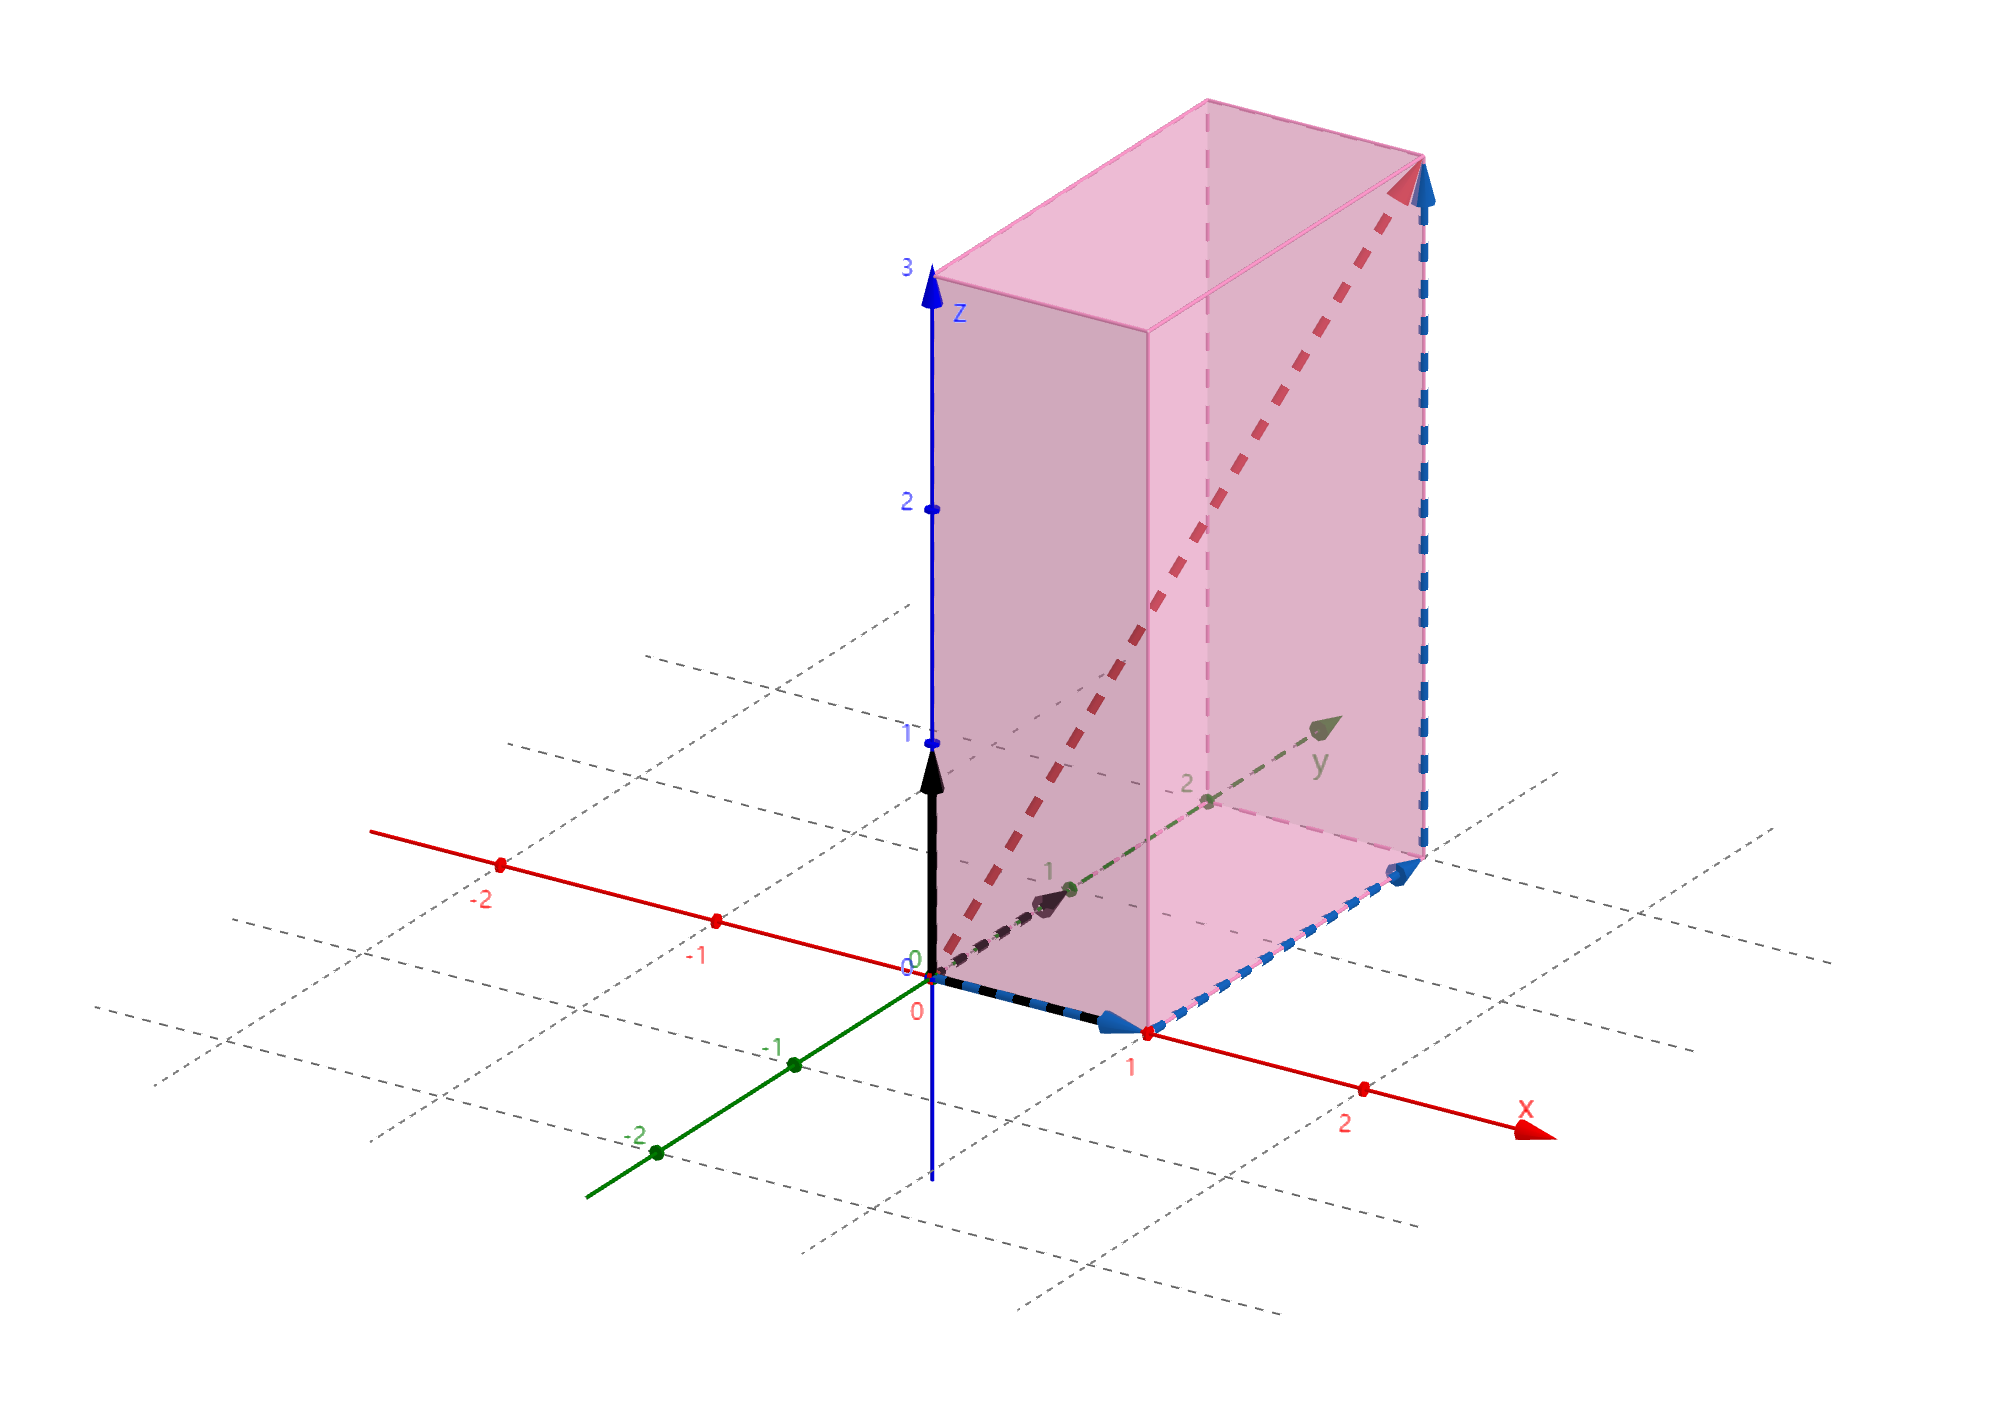
\includegraphics[width = 0.8\textwidth]{linear equation 1.png}
        \caption{向量的线性合成}
        \label{fig. linear equation 1}
    \end{figure}

    我们来说明一下这副图像所刻画的事件: 我们指定的向量 $\boldsymbol{b}$ 
    (红色) 被我们用三个所给的向量 (黑色) 以某种方式 (蓝色) 合成了. 
    向量的合成自然是高中就已经完全掌握的方法, 而我们更进一步, 我们能够组合出 
    $\boldsymbol{b}$ 是为什么呢? 怎样的向量组才能够组合出 $\boldsymbol{b}$ 
    呢? 我们可以从这个粉红色的六面体得出想法, 实际上, 我们的向量组 
    $\boldsymbol{e_1},\boldsymbol{e_2},\boldsymbol{e_3}$ 完全能够合成出
    六面体区域里的任何一个向量, 而这个粉红色的六面体能够正如向量组合上前面那个
    系数一样不断地扩张, 直到盖住整个 $\mathbb{R}^3$ 空间. 
    
    \noindent \textbf{Case 2}

    \begin{equation}
        \begin{pmatrix}
            1 & 2 & 1 \\
            1 & 0 & 3 \\
            -1 & 1 & 0 \\
        \end{pmatrix}
        \begin{pmatrix}
            x \\
            y \\
            z \\
        \end{pmatrix}
        =
        \begin{pmatrix}
            1 \\
            2 \\
            3 \\
        \end{pmatrix}
        \end{equation}
        \begin{equation}
            x
            \begin{pmatrix}
                1 \\
                1 \\
                -1 \\
            \end{pmatrix}
            +
            y
            \begin{pmatrix}
                2 \\
                0 \\
                1 \\
            \end{pmatrix}
            +
            z
            \begin{pmatrix}
                1 \\
                3 \\
                0 \\
            \end{pmatrix}
            =
            \begin{pmatrix}
                1 \\
                2 \\
                3 \\
            \end{pmatrix}
        \end{equation}

    如今方程没有那么简单了 (至少一眼望不到答案), 也很容易能够看出 
    (\ref{eq. orthonormal basis}) 的关系, 彼此相互不正交. 
    我们来直接看看它们是否能够覆盖整个空间. 

    \begin{figure}[hbtp]
        \centering
        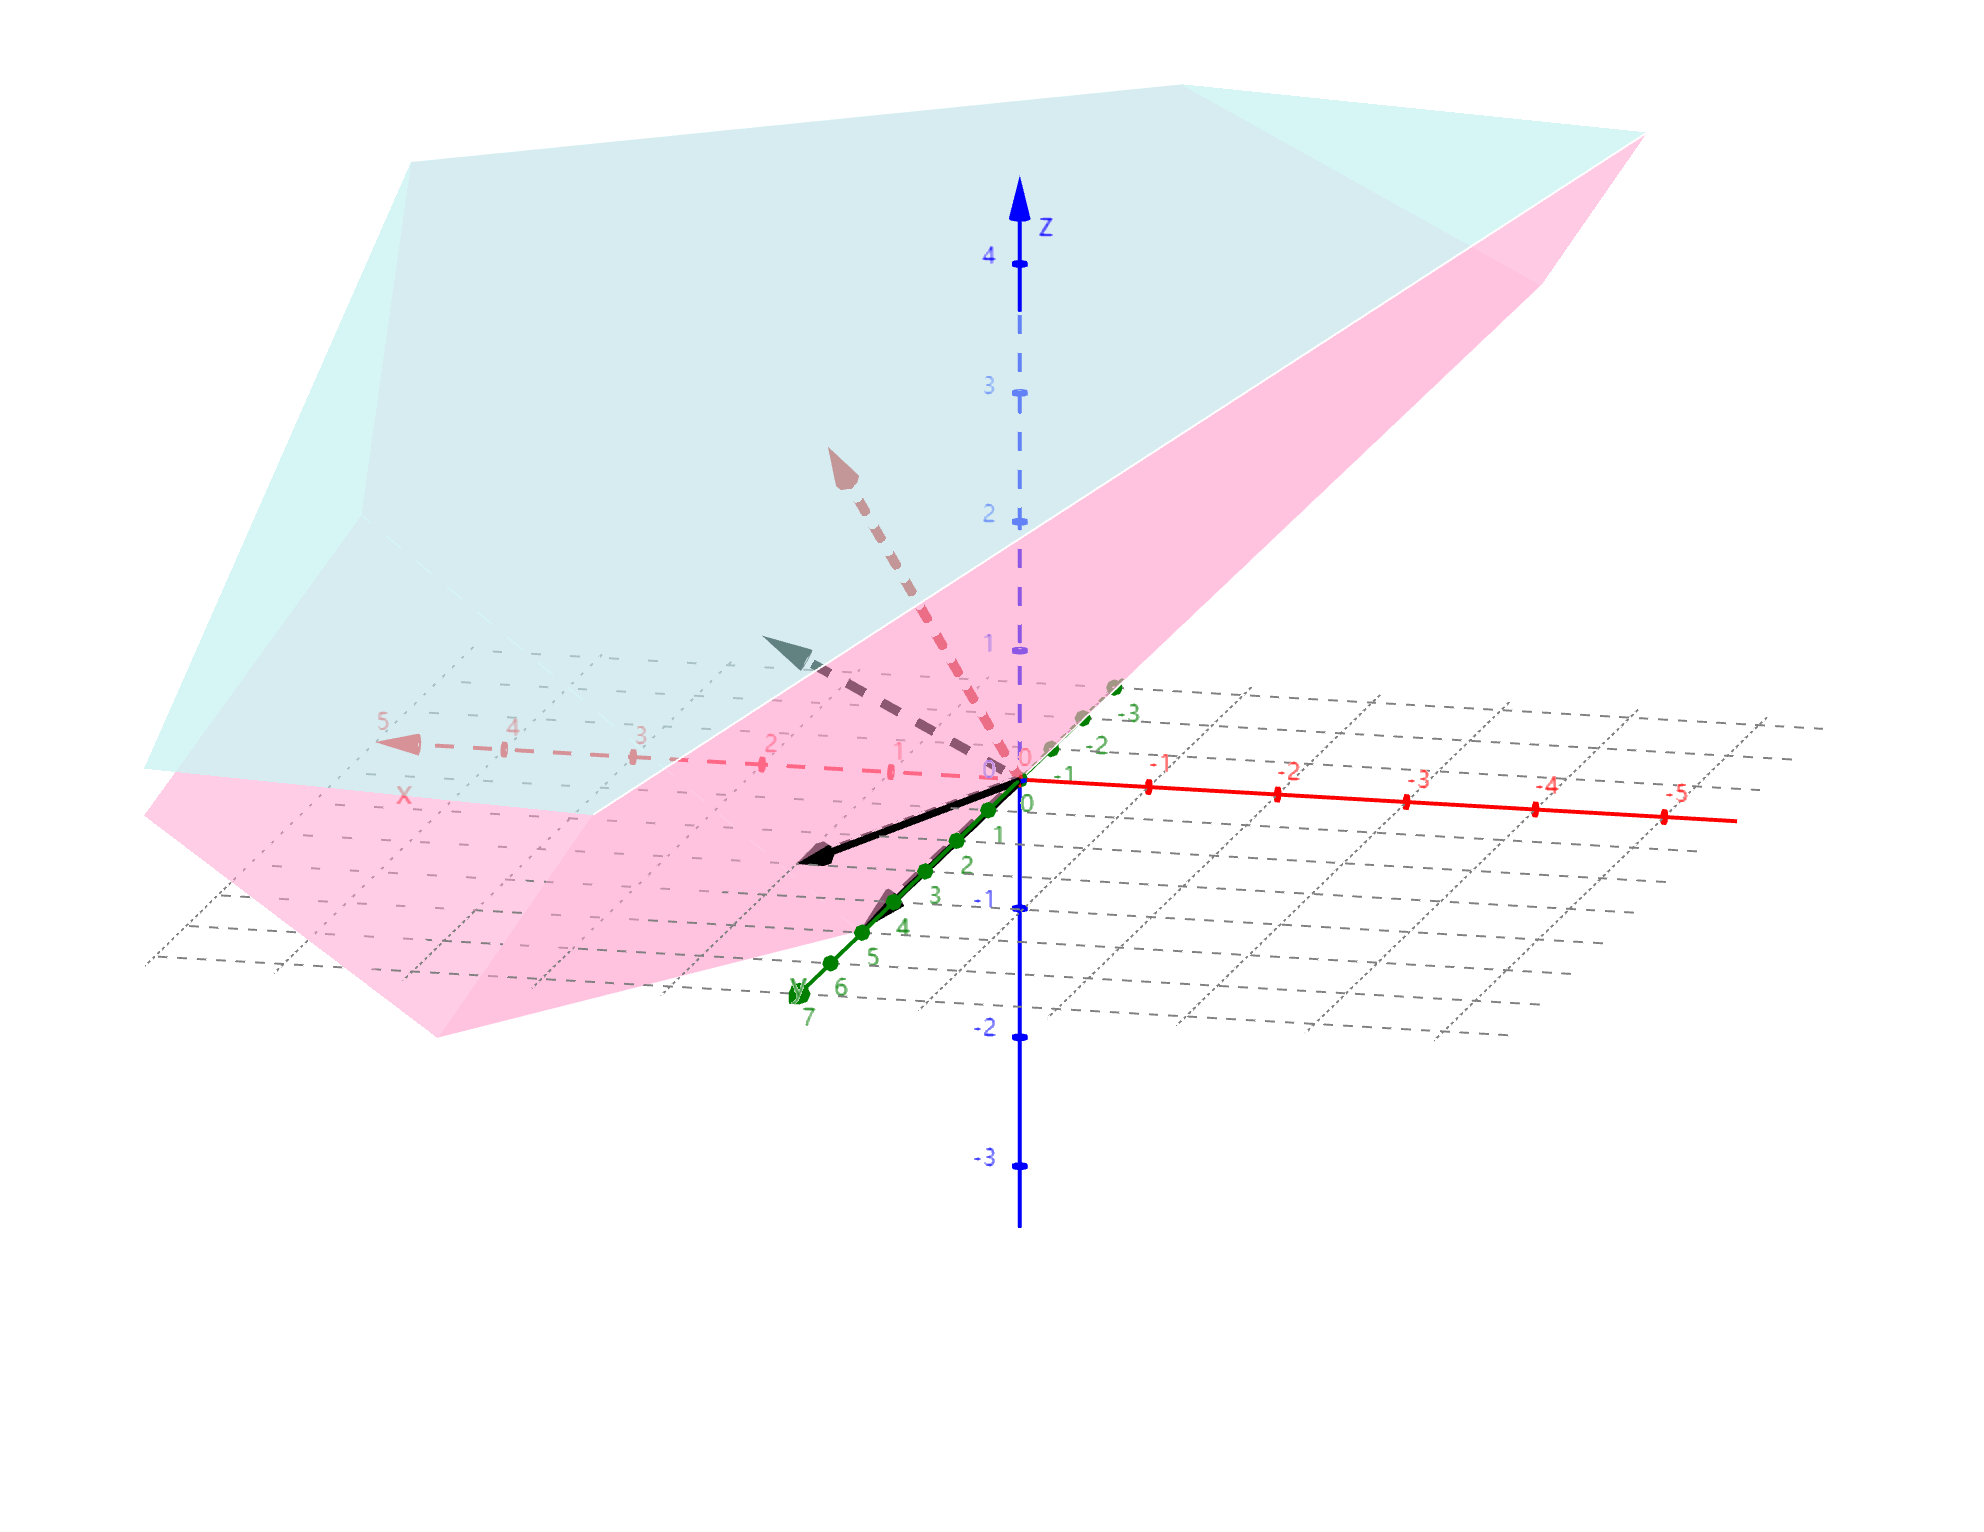
\includegraphics[width = 0.8\textwidth]{linear equation 2.png}
        \caption{向量的线性合成}
        \label{fig. linear equation 2}
    \end{figure}
    我们能够看到, 答案是肯定的, 即使这组向量并不是标准正交基, 它依旧能够覆盖
    整个空间.

    事实上, 我们更加愿意进行这样的操作, 我们会对增广矩阵
    \begin{equation}
        \begin{pmatrix}
            1 & 2 & 1 & 1 \\
            1 & 0 & 3 & 2\\
            -1 & 1 & 0 & 3\\
        \end{pmatrix}
    \end{equation}
    进行初等行变换, 将其化为 (笔者此时使用了 MATLAB 来计算这个随手写下的式子)
    \begin{equation}
        \begin{pmatrix}
            1 & 0 & 0 & -17/8 \\
            0 & 1 & 0 & 7/8\\
            0 & 0 & 1 & 11/8\\
        \end{pmatrix}
    \end{equation}
    我们再用向量语言来说明这件事, 设此时的系数矩阵有如下的向量分块 
    $\boldsymbol{A_2} = (\boldsymbol{\alpha_1},
    \boldsymbol{\alpha_2},\boldsymbol{\alpha_3})$ 
    并且进行的初等行变换对应的可逆矩阵为 $\boldsymbol{P}$, 
    则我们所做的是 
    \begin{equation}
        \boldsymbol{P}\boldsymbol{A_2} = (\boldsymbol{\alpha_1},
        \boldsymbol{\alpha_2},\boldsymbol{\alpha_3},\boldsymbol{b}) =
        (\boldsymbol{e_1},\boldsymbol{e_2},\boldsymbol{e_3},
        \boldsymbol{P}\boldsymbol{b})
    \end{equation}
    我们用一个可逆矩阵将一组向量变换成了标准正交基, 那么自然就可以覆盖全空间, 
    这正是我们熟悉的 Gauss - Jordan 消元法的意义. 
    
    等等? 我们刚才做了一件怎样的事? 我们让一组并非标准正交基的向量组覆盖了整个
    空间, 并且每一个向量都能被这个向量组唯一地表示出来. 
    而我们目前对 $\mathbb{R}^3$ 的利用中, 也从未使用过 "正交" 的方法, 
    所以, 既然如此, 我们为何就不能让 $(\boldsymbol{\alpha_1},
    \boldsymbol{\alpha_2},\boldsymbol{\alpha_3})$ 成为我们的标准正交基呢? 
    
    这就是线性空间中 "基 (basis)" 的概念.  

    而变换矩阵 $\boldsymbol{P}$ 所做的, 就是让我们的基 
    $(\boldsymbol{\alpha_1},
    \boldsymbol{\alpha_2},\boldsymbol{\alpha_3})$ 
    变换成 $ (\boldsymbol{e_1},\boldsymbol{e_2},\boldsymbol{e_3},
    \boldsymbol{P}\boldsymbol{b})$, 
    并且正如我们所希望的最好情形, 这种变换是 1-1 的. 

    \begin{exercise}
        证明 $\mathbb{R}^3 $ 中的线性变换 
        $ A: \mathbb{R}^3 \to \mathbb{R}^3 $ 
        $\boldsymbol{\alpha} \mapsto \boldsymbol{A}\boldsymbol{\alpha} $ 
        是一个 1-1 映射当且仅当 $\boldsymbol{A}$ 是一个可逆矩阵.
    \end{exercise}

    矩阵于线性空间的意义下为线性映射. 

\noindent \textbf{Case 3}
\begin{equation}
    \begin{pmatrix}
        1 & 1 & 1 \\
        0 & 1 & 2 \\
        0 & 2 & 4 \\
    \end{pmatrix}
    \begin{pmatrix}
        x \\
        y \\
        z \\
    \end{pmatrix}
    =
    \begin{pmatrix}
        1 \\
        2 \\
        3 \\
    \end{pmatrix}
    \end{equation}
    \begin{equation}
        x
        \begin{pmatrix}
            1 \\
            0 \\
            0 \\
        \end{pmatrix}
        +
        y
        \begin{pmatrix}
            1 \\
            1 \\
            2 \\
        \end{pmatrix}
        +
        z
        \begin{pmatrix}
            1 \\
            2 \\
            4 \\
        \end{pmatrix}
        =
        \begin{pmatrix}
            1 \\
            2 \\
            3 \\
        \end{pmatrix}
    \end{equation}
    我们来直接看看它们组成的空间是怎样.

    \begin{figure}[h]
        \centering
        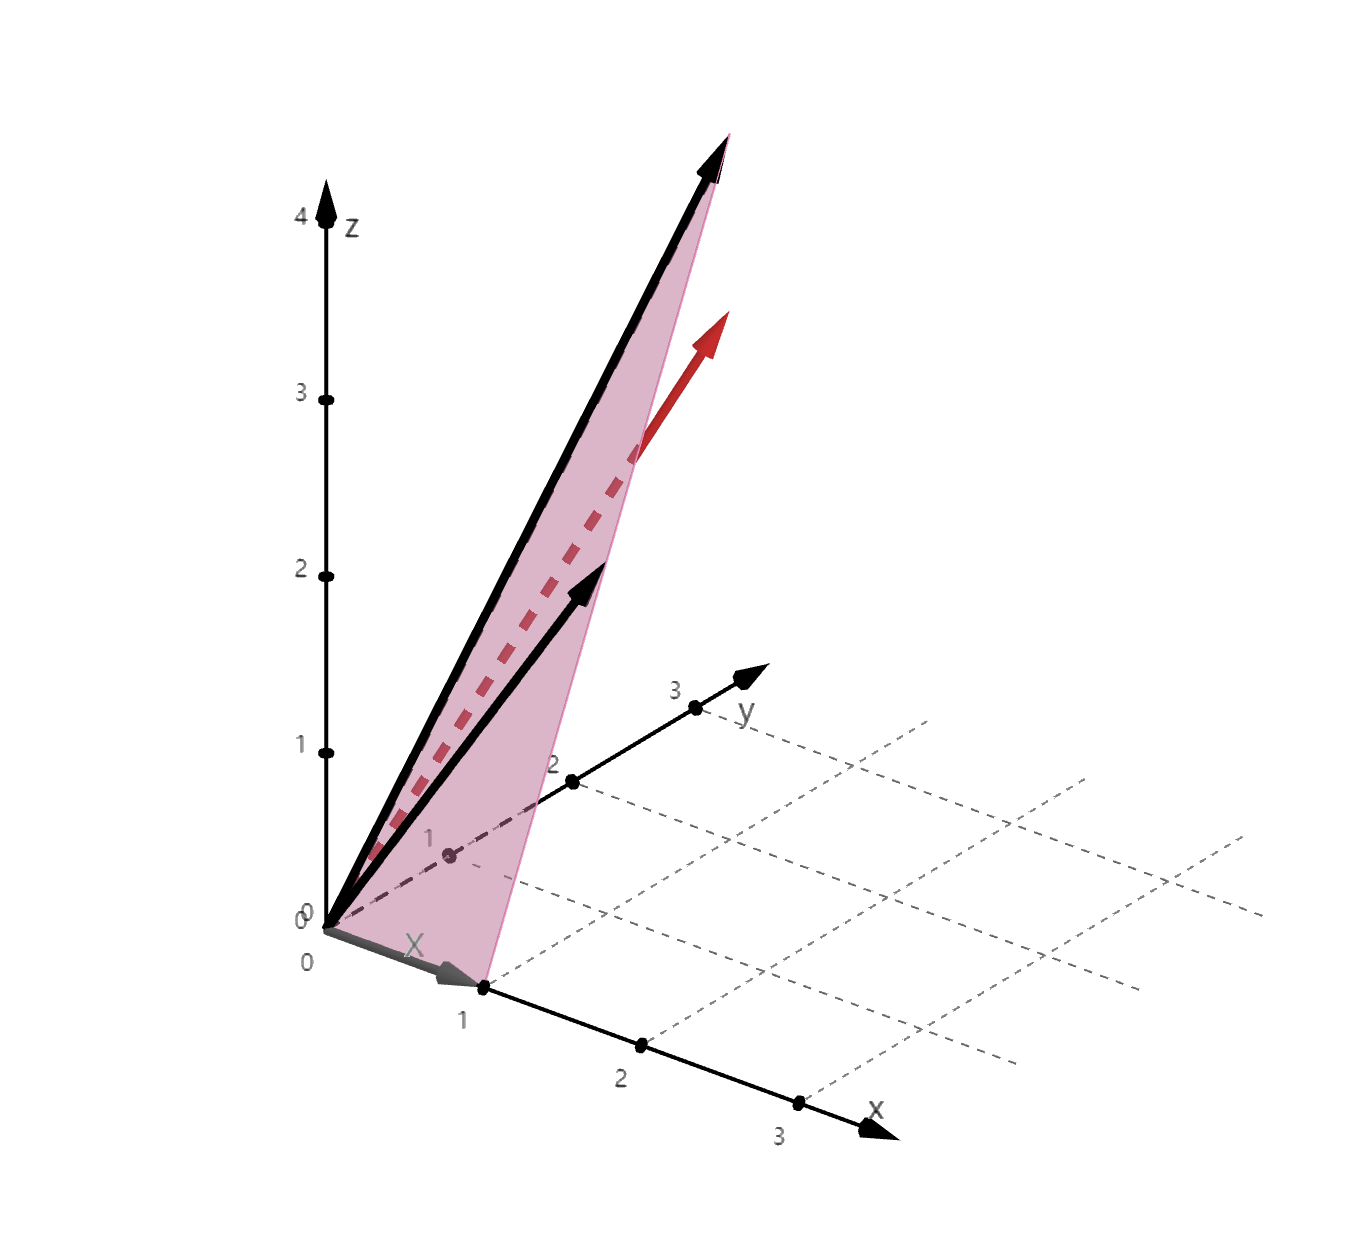
\includegraphics[width = 0.5\textwidth]{linear equation 3.png}
        \caption{向量的线性合成}
        \label{fig. linear equation 3}
    \end{figure}
    
    如图所见, 此时我们的向量组 $\{\boldsymbol{\alpha_1},
\boldsymbol{\alpha_2},\cdots, \boldsymbol{\alpha_n}, \}$ 
    只能够组成一张平面, 而由于我们的非齐次项 $\boldsymbol{b}$ 并未
    在这张平面内, 所以此时方程是无解的. 
    换句话来说, 我们也并非要求向量组 $\{\boldsymbol{\alpha_1},
\boldsymbol{\alpha_2},\cdots, \boldsymbol{\alpha_n}, \}$ 
    一定能够覆盖整个空间, 我们对它的要求是向量 $\boldsymbol{b}$ 可以
    被向量组 $\{\boldsymbol{\alpha_1},
\boldsymbol{\alpha_2},\cdots, \boldsymbol{\alpha_n} \}$ 线性表出. 

事已至此, 我们用我们现在所观察到的现象, 来简述一下线性方程组
解的存在唯一性理论吧. 

对于一个 $m$ 个方程 $n$ 个未知量的非齐次线性方程组 
$\boldsymbol{Ax}=\boldsymbol{b}$, 我们将系数矩阵
$\boldsymbol{A}$ 进行列分块 
$\boldsymbol{A}=\boldsymbol{\alpha_1,\alpha_2,\cdots,\alpha_n}$ 
后我们转化成一个等价的 "线性向量方程" 
\begin{equation}
    x_1 \boldsymbol{\alpha_1} + x_2 \boldsymbol{\alpha_2} +
    \cdots + x_n \boldsymbol{\alpha_n} = \boldsymbol{b}
\end{equation}
其中 $x_i \in \mathbb{R}$, $\boldsymbol{\alpha_i}\in \mathbb{R}^m$, 
$i =1,2,\cdots,n$. 

我们再引入一个记号 $$L(\boldsymbol{\alpha_1},
\boldsymbol{\alpha_2},\cdots, \boldsymbol{\alpha_n})
:= \{x_1 \boldsymbol{\alpha_1} + x_2 \boldsymbol{\alpha_2} +
\cdots + x_n \boldsymbol{\alpha_n}: \forall x_i \in \mathbb{R}, 
i=1,2,\cdots n\}$$ 
表示由向量组 $\{\boldsymbol{\alpha_1},
\boldsymbol{\alpha_2},\cdots, \boldsymbol{\alpha_n} \}$ 
\textbf{生成的向量 (线性) 空间}. 
那么, 我们说方程 $\boldsymbol{Ax}=\boldsymbol{b}$ 有解指的就是 
$\boldsymbol{b} \in L(\boldsymbol{\alpha_1},
\boldsymbol{\alpha_2},\cdots, \boldsymbol{\alpha_n}) $. 

齐次线性方程组是非齐次线性方程组的一个特殊情况, 当我们取 
$\boldsymbol{b} = 0$ 时, 我们必然有一个解 $x_1 = x_2 =\cdots= x_n = 0$. 
因此我们对齐次线性方程组只分析解的唯一性. 

接下来我们再分析解的唯一性. 

假设 $\boldsymbol{b} $ 在 $L(\boldsymbol{\alpha_1},
\boldsymbol{\alpha_2},\cdots, \boldsymbol{\alpha_n})$ 中有两个线性表示, 
分别记为 $\boldsymbol{X}=(x_1,x_2,\cdots,x_n)$ 和 
$\boldsymbol{Y} = (y_1,y_2,\cdots,y_n)$ 
指代的是它们和向量组的乘积即 $(\boldsymbol{\alpha_1},
\boldsymbol{\alpha_2},\cdots, \boldsymbol{\alpha_n})X $, 
我们称这样的表示 $\boldsymbol{X}=(x_1,x_2,\cdots,x_n)$ 为在
向量组 $(\boldsymbol{\alpha_1},
\boldsymbol{\alpha_2},\cdots, \boldsymbol{\alpha_n})$ 
下的一个坐标, 于是我们要研究的唯一性就是这种坐标的唯一性. 

通过线性组合的计算方法, 我们得到一个新的齐次线性方程 
$$k_1 \boldsymbol{\alpha_1} + k_2 \boldsymbol{\alpha_2} +
\cdots + k_n \boldsymbol{\alpha_n} = 0$$ 其中 $k_i = x_i - y_i, \,
i = 1,2, \cdots ,n$. 
于是, 只要通过这个线性组合的式子可以得到 
$ k_1 = k_2 = \cdots = k_n = 0 $ 我们就得到了解的唯一性. 
这正是\textbf{线性无关}所保证的. 

拥有了线性无关, 我们再来回头看看存在性. 

我们之前说的解不存在, 其实也就是说 $\boldsymbol{b}$ 无法被线性表出. 
那么自然可以得到 $L(\boldsymbol{\alpha_1},
\boldsymbol{\alpha_2},\cdots, \boldsymbol{\alpha_n}) \neq
L(\boldsymbol{\alpha_1},
\boldsymbol{\alpha_2},\cdots, \boldsymbol{\alpha_n},\boldsymbol{b})$. 
用我们之前所学的语言来说, 前一组向量组的极大无关组向量个数
比后者多 1 个.



\subsection{Grassmann 与《扩张论》}

\songti
以下选自 John Derbyshire -《代数的历史: 人类对未知量的不舍追踪》. 
这本书可以算是最好的代数学历史书. 
\vspace*{0.8cm}

\kaishu
这一时期, 在普鲁士的斯德丁 (现在波兰的什切青) 有一位名叫赫尔曼・甘特・格拉斯曼的中学校长. 
1843 年时他 34 岁,从 1831 年开始他一直在这个高中任教, 一辈子都在教书育人. 
他的数学是自学的, 他在大学时学的是神学和哲学. 他 40 岁结婚, 有 11 个孩子.


哈密尔顿发现四维向量空间的第二年, 格拉斯曼出版了一本名字很长的书 ——《…线性扩张论》, 
通常我们叫作《扩张论》. 在这本书中, 格拉斯曼研究了 80 年后才出现的向量空间理论. 
他定义了一系列概念, 诸如线性相关、线性无关、维度、基、子空间和投影. 事实上, 
不仅如此, 他还给出了向量乘积的方法和代表基的变换方法, 
因此也就用比哈密尔顿的四元数更通用的方法发明了 "一个代数" 的概念. 
所有这一切都是按很强的代数风格完成的, 强调了这些新数学对象完全抽象的属性, 
仅仅是作为这些代数对象的应用引入了几何的思想. 

但是, 格拉斯曼的书几乎没有得到关注. 只有格拉斯曼自己写了一篇评论. 事实上, 格拉斯曼就如阿贝尔、
拉芬尼、伽罗华等这些非常悲哀的数学家一样, 他们的价值不会被同代人接受. 
另外,也有他自己的问题. 他的著作《扩张论》的写作风格按 19 世纪初的习惯充满了形而上学的色彩, 
令人难以理解. 莫比乌斯对它的描述是 "无法阅读", 尽管他尝试着帮助格拉斯曼, 
并于 1847 年写了一篇评论赞扬了格拉斯曼的想法. 格拉斯曼全力推销这本书, 
但是他运气不好,没人理睬. 
法国数学家圣维南 1845 年发表了一篇关于向量空间的论文. 
这是《扩张论》出版后的第二年. 尽管圣维南与格拉斯曼不认识, 
但他的这篇论文展示了与格拉斯曼类似的想法. 读了这篇论文后, 
格拉斯曼把《扩张论》中的相关段落寄给了圣维南. 但他不知道圣维南的地址, 
只好通过法国科学院的柯西转交, 并请求柯西尽快送到. 然而, 柯西没有这样做, 
并且于 6 年后发表了一篇论文, 这篇论文非常有可能源自格拉斯曼的著作. 
格拉斯曼向科学院提出了抗议. 尽管科学院成立了三人委员会来调
查是否发生了剽窃,但最终没有得出任何结论……

《扩张论》也并非完全不可读. 
哈密尔顿就于 1852 年看了这本书, 并在其著作《四元数讲义》的引言中对格拉斯曼
做了短评. 他赞扬《扩张论》是 "原创和杰出的", 但是强调他自己的方法不同于
格拉斯曼的方法. 就这样, 格拉斯曼的著作出版 9 年后, 有两位认真严谨的科学家注意到了
它: 莫比乌斯和哈密尔顿. 
格拉斯曼尝试着重写《扩张论》, 使它更容易被人接受,并于 1862 年自己出资出版了新版本, 
共有 300 页. 这一新版本的前言中有如下一段话, 我觉得它相当感人. 


\begin{quotation}
    \textsf{
    我始终坚信我在此科学上所付出的劳动不会白费, 它耗尽了我生命中最重要的阶段, 
    让我付出了超常的努力. 我当然知道我给出的这门科学的形式还不完善, 
    它一定是不完善的. 但是, 我知道而且有义务在此声明 (可能有人会认为我很狂妄), 
    即使这一成果再过十七年或更长时间还不被使用, 也没有真正融入到科学的发展之中, 
    它冲出遗忘的尘埃现身的时候也一定会到来, 现在沉睡着的思想结出硕果的那一天一定会到来. 
    我知道, 如果我今天还不能 (如我至今徒劳地期望那样) 把学者们吸引到我的周围, 
    用这些思想帮助他们成果累累, 促使其进步, 丰富其学识, 
    那么这种思想在将来一定会重生, 或许以另一种新形式, 与时代发展水乳交融. 
    因为真理是永恒不灭的. 
    }
\end{quotation}

1862 年版的境遇比 1844 年的稍好些. 然而, 由于理想的破灭, 格拉斯曼不再研究数学, 
而是投身于梵语研究. 他出版了一本大部头的翻译著作, 把梵语的经典著作《梨俱吠陀》翻译成德语, 
附加上很长的注释, 总共有 3000 页. 因为这一成就, 
他获得蒂宾根大学授予的荣誉博士称号. 

直接以格拉斯曼的工作为基础的第一个重要的数学进步发生在 1878 年, 
这时他已经去世一年了. 
当时英国数学家克利福德发表了一篇题为《格拉斯曼扩展代数的应用》的论文. 
克利福德利用格拉斯曼的想法把哈密尔顿的四元数一般化成为 n 维代数族. 
后来证明这些克利福德代数可以用于 20 世纪的理论物理. 
n 维空间内的旋转 (即旋子的现代理论) 就来自于它们.

\vspace*{0.8cm}

\songti
笔者个人非常喜欢 Grassmann 这段话, 并希望将这段话送给每个热爱数学的人. 
请别忘了最根本的热爱, 在这一路的途中. 



\end{document}
